\scanpage{130}%
% archive sheet number: 129
% source lines 1--2; completes préliminaire from scan 129
minary, - with at most the proviso that there exists such an $\unsure{\mathbb{E}|\mathbb{F}|E|F}$ over a suitable extension of $k_x$ (something perhaps always tru\handwritten{e}).

% source lines 3--12
12. \uline{Instructive examples}. Let $G$ be a finite \unsure{\(\mathbb m\)|\rlap{a}m|\rlap{u}m}onoid. Contrary to the general Galois yoga, instead of taking $A=k(G)$ (ring of functions on the underlying set of $G$) let us take $U=k(G)$, with th\deleted{a}e diagonal map deduced from $GxG\handwritten{\longrightarrow}G$ (the composition). (We have the ``d\unsure{\rlap{a}u|u|a}al'' bialgebra \inserted{in Cartier's sense} of the one usually considered). Thus the category $C$ defined by $G$ \deleted{is} can be considered as the category of families $(\unsure{\rlap{\(M\)}X|\mathbb M|\mathbb X}_g)_{g\ G}$ of vector spaces indexed by $G$, th\unsure{\rlap{'}e|é|e} \deleted{diagonal map} \inserted{tensor} product of two such $X$ and $Y$ being $Z$ defined by $Z_g=\handwritten{\displaystyle\sum}_{g'g''=g}X_{g'}\unsure{\otimes|\Omega} Y_{g''}$. The unit is the ``Dirac family'' defined by $\rlap{\(M\)}X_g=0$ if $g\handwritten{\ne}\mathbb{e}$, $\rlap{\(M\)}X_e=k$.\inserted{We have a \unsure{\rlap{c}C|\(\mathbb C\)|C|c}ategory with $\otimes,\handwritten{\phi},1$, and moreover a $\handwritten{\unsure{\psi|\mu}}$ if $G$ is commutative, a $\handwritten{\vee}$ if $G$ is a group.}

% source lines 13--24, with one displayed formula and its right marginal note
An $L$ with a diagonal map $L\handwritten{\longrightarrow}L\otimes_k L$ compatible with $U\handwritten{\to}U\otimes_k U$ and giving an isomorphism by extensions of the base rings, can be interpreted as a family $(\deleted{M}\handwritten{L}_g)_{g\handwritten{\in}G}$, with given isomorphisms
\[
(\unsure{\rlap{\(x\)}-|*})\qquad \deleted{M}\handwritten{L}_{gg'}\handwritten{\simeq}\deleted{M}\handwritten{L}_g\otimes\deleted{M}\handwritten{L}_{g'}\ .
\]
\margin{This implies that the rank of the $\deleted{M}\handwritten{L}_g$ is $0$ or $1$}
It is compatible with $1$ if we have an isomorphism\inserted{\handwritten{\unsure{(*+)|(**)}}}\handwritten{\begin{tikzpicture}[x=.2cm,y=.2cm,baseline=-.1ex]\draw (0,-.5) .. controls (.2,.1) and (1,.2) .. (1.5,.8);\end{tikzpicture}} $\deleted{M}\handwritten{L}_e\handwritten{\simeq}k$, which make\deleted{r}s the isomorphisms $(\rlap{\(x\)}-)$ trivial when \deleted{these} $g$ or $g'$ is $=1$. It is associative if and only if the isomorphisms $(\rlap{\(x\)}-)$ satisfy the \deleted{conditio} obvious associativity conditions. Likewise, $G$ being commutative, for commutativity. - The functor $F'$ is always exact, since $M$ is flat over $U$.

% source lines 25--30
a) Example of an exact $\otimes$-functor, compatible with $\handwritten{\phi,\psi},1$, \uline{but not faithful} (thus not locally iso\unsure{\rlap{m}M|M|m}orphic to the given $\otimes$-functor). This is possible in our example only if $G$ is not a group (\deleted{otherwise $M$} since $\deleted{M}\handwritten{L}_g$ is of rank $1$ for $g$ invertible). But let us take $G=(e,p)$, with $p^2=p$, let us take $\deleted{M}\handwritten{L}_e=k$, $\deleted{M}\handwritten{L}_p=0$. We no longer have a choice for the isomorphisms $\rlap{\(x\)}-$, which satisfy all the compatibilities (with $1_x$ by construction, $\handwritten{\phi,\psi}$).
% bottom margin, below a handwritten separating rule
\figure{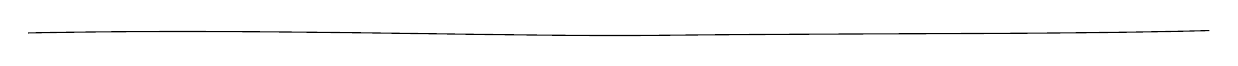
\begin{tikzpicture}[x=1cm,y=1cm]\draw (0,.03) .. controls (3,.09) and (6,-.02) .. (8,0) .. controls (11,.03) and (13,.01) .. (15,.06);\end{tikzpicture}}
\margin{\handwritten{\uline{Question} Is a $\otimes$-functor compatible with everything between $\otimes$-categories satisfying all the axioms (including rigidity) necessarily faithful and exact ?!}}
